\chapter*{Motivation}
\addcontentsline{toc}{chapter}{Motivation}
In order to track and follow up project's status, my colleagues and I
built, on 2013, a simple tool in a spreadsheet that linked with a database that
allowed us to log each change (aka \emph{event}) on the project status of on
the following scope: phase change end/start, delay, launch.

This tool also gave us a good view about different selected KPI \footnote{Key
Performance Indicator}. And based on those indicators some reports can be
built:
Project's events, Project's launched, Project's delayed (and detail), Project's
Gantt and Project's timelines.

The tool was fine for a while, but it took too much time to load all data
from the database, and also was not fully accessible for all users, because
of the need to install some extra required components like the ODBC for those with
Windows, or not even compatible with those using Linux computers, because the
tool was built on Microsoft Excel.

So, imagine trying to track project's \emph{events} on a tool that is slow
and not compatible with everybody. At the end we stopped using it.

Then, a fresh motivation came up to build something better,
usable for all required users and faster enough to aim the objective: track,
analyze and decide. 

The challenge was both there and as well the information on the database, so it
was just a matter to migrate the spreadsheet (the view) to a HTML page with some JS,
as first client, so we decouple it from any need of 3rd party component such as
ODBC, having in the middle a RESTful service that
controls the communication between the client (web browser) and what matters,
the data (our business).

\part{Migrate Excel spreadsheet dashboard to a simple REST+HTML/JS
application}
\label{c_phaseone}

\chapter{Current Excel architecture}
At the beginning, the idea was to have the data centralized
\label{t_main_objective} and implement, in a fast way, a client that could show
it. The quickest solution, not always the right one but useful for a while, was
to define the simplest database model to  track the maximum amount of events
with enough value to evaluate the  efficiency of a project and learn from our
mistakes.

Together with the database  we setup an Excel spreadsheet that loaded
the data from the defined database, but  we also needed to build different
reports, so we defined few \emph{views} based  on the required KPIs, so we could
query it from the external spreadsheet  without defining any kind of logic,
that could increase the complexity.\\ 

In short, elements defined are listed as follow:
\begin{itemize}
  \item A MySQL database with one table called Events used to store any possible
  event (previously defined the set of them)
  \item Few views used to achieve defined reports
  \item A Microsoft Excel spreadsheet used to show data returned by the views
  \item One connection per report used to connect Excel with the database
  via ODBC as data connectivity abstractor. 
\end{itemize}

You can see the relationship between above listed components on the 
\reffigure{f_excel_architecture}.
 
\begin{figure}[ht!]
	\centering
   	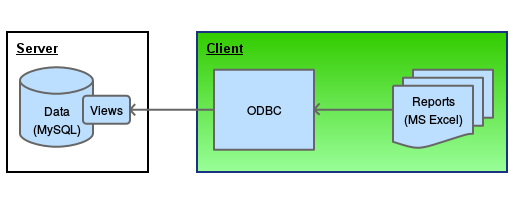
\includegraphics[width=1\textwidth]{./resources/excel_architecture.png}
   	\caption{Reports architecture using Excel}
   	\label{f_excel_architecture}
\end{figure}

\section{Database model}
The database model was defined as simple as possible, keeping in mind
possible normalization in the future without having a big impact on the data. So
decision was to use
\emph{Enum}\footnote{\url{https://dev.mysql.com/doc/refman/5.0/en/enum.html}}
data type for those fields that are static or with a predefined set of
elements like: country, project\_type or  type fields
(\reffigure{f_data_model}).

\begin{figure}[ht!]
	\centering
   	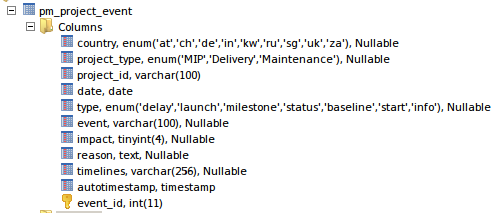
\includegraphics[width=1\textwidth]{./resources/data_model.png}
   	\caption{Data model}
   	\label{f_data_model}
\end{figure}

The most relevant field here is \emph{type}, which covers all required possible
scenarios in a project's lifetime that we needed to track. And base on that, 
reports (views) can show the specific information to be analyzed.

\section{Views definition and reports}
As described on the previous sections, we defined five reports, they are:

\begin{itemize}
  \item Amount of launches, per country and month
  \item Total project's delay
  \item Project's delays in detail
  \item Gantt chart
  \item Project's timelines chart 
\end{itemize}

On top of them, we also added an extra report listing all project's events,
just for our reference.

You can see screenshots on how they look for each of them on
\reffigure{f_report_launches}, \reffigure{f_report_delays},
\reffigure{f_report_delays_detail}, \reffigure{f_report_gantt},
\reffigure{f_report_timelines} and \reffigure{f_report_events}.

\begin{figure}[ht!]
	\centering
   	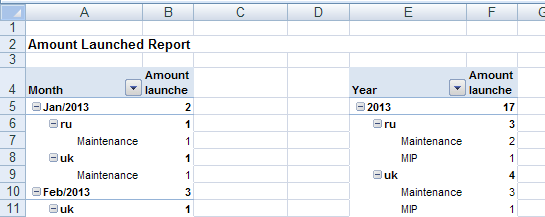
\includegraphics[width=1\textwidth]{./resources/report_launches.png}
   	\caption{Launches report}
   	\label{f_report_launches}
\end{figure}
\begin{figure}[ht!]
	\centering
   	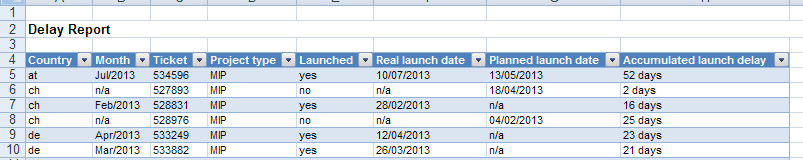
\includegraphics[width=1\textwidth]{./resources/report_delays.png}
   	\caption{Delays report}
   	\label{f_report_delays}
\end{figure}
\begin{figure}[ht!]
	\centering
   	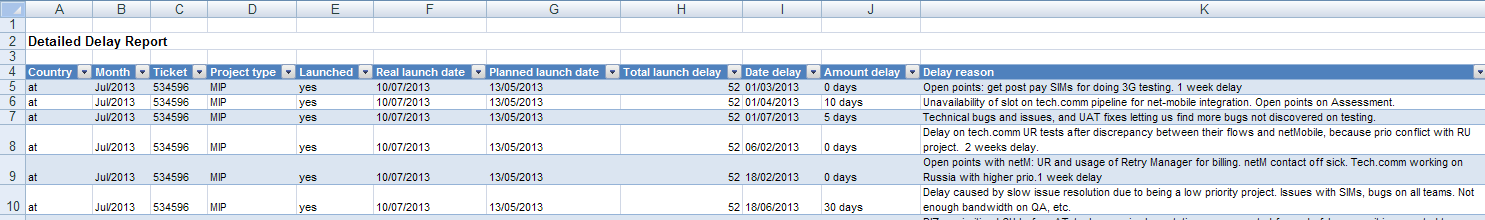
\includegraphics[width=1\textwidth]{./resources/report_delays_detail.png}
   	\caption{Detailed delays report}
   	\label{f_report_delays_detail}
\end{figure}
\begin{figure}[ht!]
	\centering
   	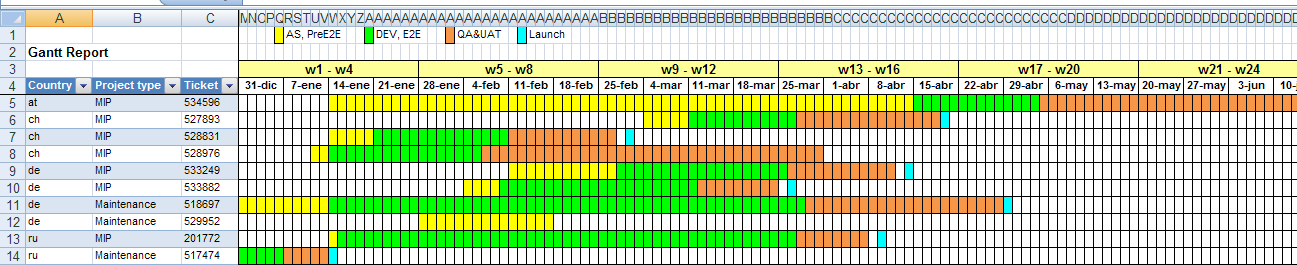
\includegraphics[width=1\textwidth]{./resources/report_gantt.png}
   	\caption{Gantt report}
   	\label{f_report_gantt}
\end{figure}
\begin{figure}[ht!]
	\centering
   	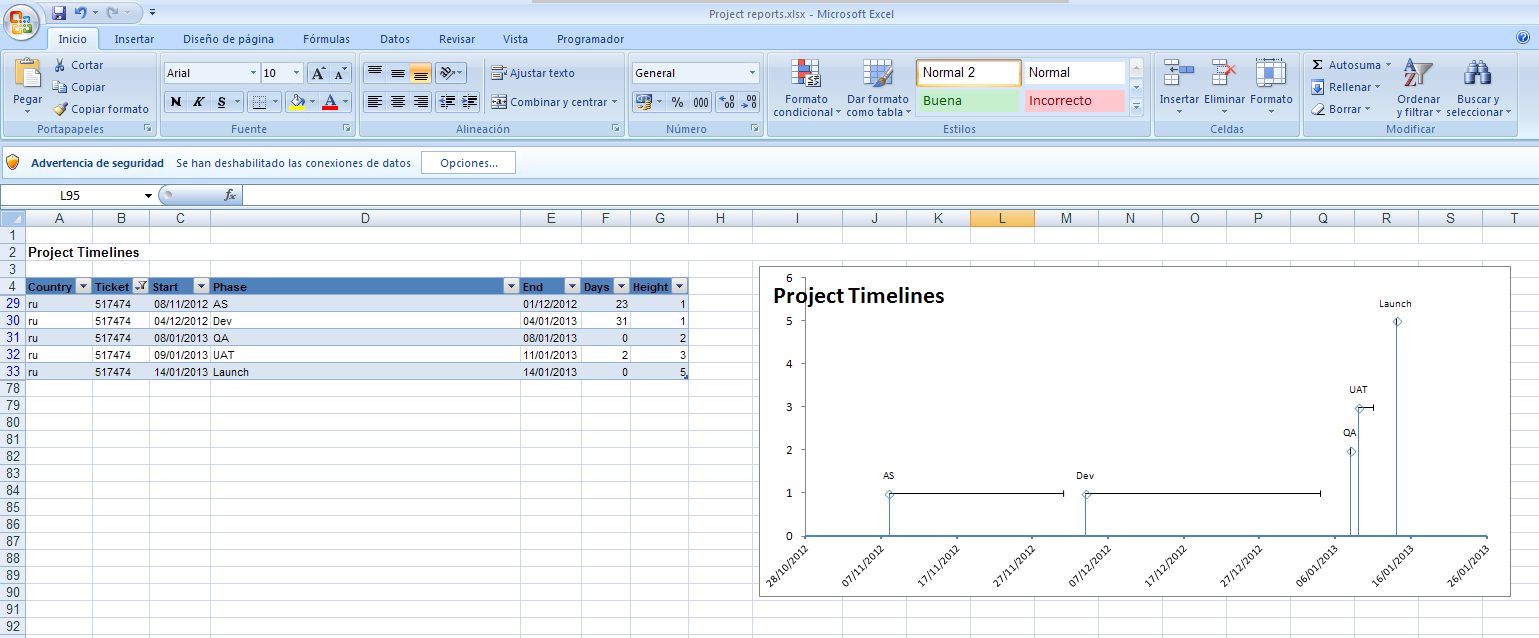
\includegraphics[width=1\textwidth]{./resources/report_timelines.png}
   	\caption{Timelines report}
   	\label{f_report_timelines}
\end{figure}
\begin{figure}[ht!]
	\centering
   	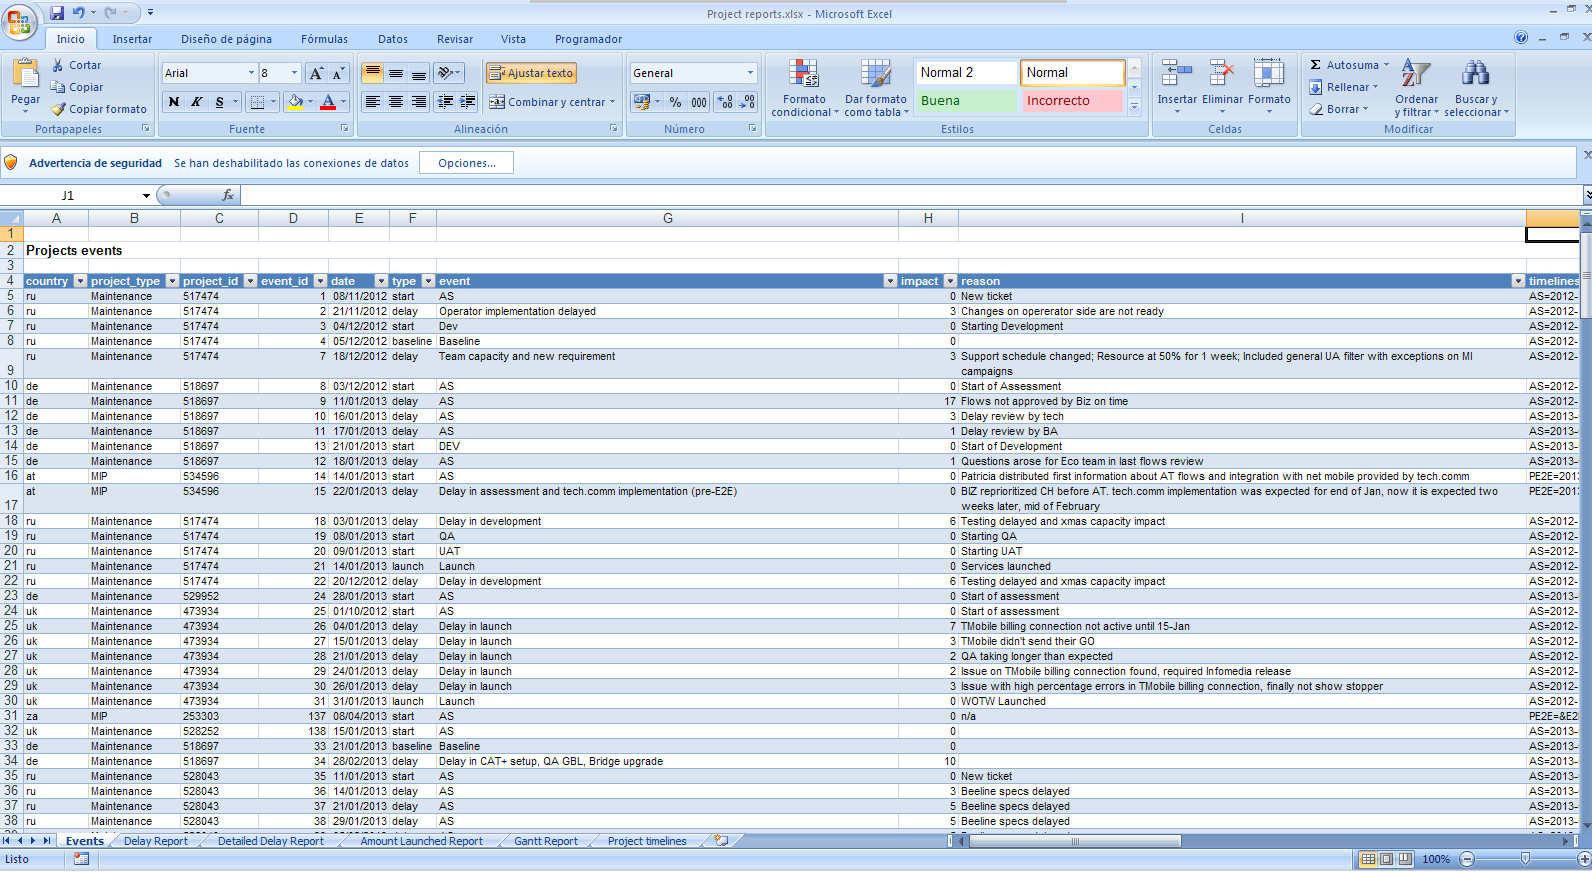
\includegraphics[width=1\textwidth]{./resources/report_events.png}
   	\caption{Events report}
   	\label{f_report_events}
\end{figure}

Each of those reports has defined one or more than one table's view that execute
the required data calculations and format the output in a Excel friendly way, so
the spreadsheet just needed to show it and didn't require any customization. 

This data and format coupling on the views definition was done on purpose,
in order to be flexible enough in the future in case defining a different viewer
component was needed, a part of the Excel, such as and HTML, or just migrate it
to a different platform. But, on both cases the model could remain untouched if
the objective remained the same and only is needed to change the  view with a
more powerful or friendly one. See an example on
\ref{f_report_launchesbymonth}, where ``Amount of Launches by Month'' query 
is defined, querying the main table \texttt{pm\_project\_event}, grouping and
counting by launch's year-month, country and project\_type.

\lstinputlisting[style=sql,caption=Launches\ by\ month\ view,label=f_report_launchesbymonth]{resources/report_launchesbymonth.sql}

On the other hand, decoupling it will be needed to be taken care sooner or
later if we want to have a flexible and scalable tool, but this will be part of the
future work.

\section{The issue and what to improve}
As slightly tackled on previous sections, building a reporting tool based on
Excel was not the best solution, but it covered the main needs, even if we
faced issues like slowness, a single shared spreadsheet to be used by all
project managers, every report had a standalone database connection with the
possible impact on resources it could have a manual database insert per
each project's event.

All these points will be reviewed and covered on the next chapter. 

\chapter{New RESTful architecture}
After few time working with the spreadsheet linked with the database, and having
listed its downsides, we have started thinking about how to improve it without
affecting the main objective \ref{t_main_objective} but making it more
user friendly.

We already had listed the weaknesses and thinking on them, just came
up that the main change would be to replace completely the view (Excel), that
will solve all the issues, but will lose the power of the pivot table and
filters, but it could be managed in a second or third stage.

Now the question is: what could be the best replacement?

\section{Looking for a view replacement}
We wanted to have a very light view and user friendly, something that
provides directly the information to the user, a dashboard where the user could
see in one single view all the information he wants to see.

Nowadays, there are good examples of dynamic data dashboards done with the
latest online technologies like
Graphite\footnote{\url{http://graphite.wikidot.com/}},
Dashing\footnote{\url{http://shopify.github.io/dashing/}} or even using Google
Charts that could provide a good
dashboard\footnote{\url{https://developers.google.com/chart/}}.  

Why online? Because today everything is connected and you can interact with
almost everything, and why not with the status of a project? Also, if you are
not connected, you are not cool and very unuseful, and we wanted to have a
useful tool, and why not, also have a cool tool!  On top of that, objective is
challenging, so better to go for a lean approach\footnote{\url{http://en.wikipedia.org/wiki/Lean\_software\_development}} and
deliver small pieces with the enough functionality even if they are not covering
the final objective. So, following this approach the first target was to have
a simple view of what we are managing here, projects and dates. So using Google
Charts we have enough to start and close the first phase. Also using a very
plain HTML and CSS code to provide the simplest functionality to enter the
required data.

\section{Looking for a REST server}
Once we have clear what is the view, we can start thinking about what could be
the best option to process the data we are going to use on the view.

We already knew that the architecture was going to be a server-client one and
mostly using REST approach in order to minimize the coupling between the
components, but there are many frameworks and web servers that provide this
functionality and further more, so what could fit better on our model?

One think we had very clear is we were looking for a Java implementation, why?
Because it provides a big amount of possible frameworks and technologies to
use or plug in and also maybe because we am more familiar and confident
with it.

Within the big umbrella of available Java servers\footnote{\url{http://en.wikipedia.org/wiki/Comparison\_of\_application\_servers\#Java}},
we found Jersey\footnote{\url{https://jersey.java.net/}}, a
RESTful framework implemented in Java, that covers the following
requirements:
\begin{itemize}
  \item Java environment
  \item Compatible with Java containers such as Apache Tomcat 
  \item Extensible and scalable
  \item Compatible with JAX-RS
  \item Easy to use out of the box
\end{itemize}

There were other available options, such as
Restlet\footnote{\url{http://restlet.com}} or
RESTEasy\footnote{\url{http://resteasy.jboss.org/}}. All three options fit our
needs, but we decided to use Jersey just to try it, but all three (and others)
frameworks are good enough so far, so we just needed to pick one and try it.

A part of the REST framework, we also found too Grizzly\footnote{\url{https://grizzly.java.net/}} as a Server application, that will
provide to or tool a better scalable future in case we need it taking
advantage of Java NIO\footnote{\url{https://www.jcp.org/en/jsr/detail?id=51}}.
Both Jersey and Grizzly are Oracle projects.

Now that seems that we have everything in place, we can start to open Eclipse
and start typing the code that will replace the spreadsheet. But this will be
part of the migration plan described on the following chapter.

\chapter{Migration}
Do not forget that the target is to deliver a \emph{simple} tool that replaces
current Excel, so the migration will start developing the minimum code in order
to add, update and delete project's events and also provide the same
information that currently to the view in order to show it.

Considering also that we are not familiar with Grizzly and Jersey, the first
thing we will need to deploy is a very simple server and REST application,
using the examples, in order to understand the logic and the process. You can find all the
information on the project web page as well the tutorials and the examples that
will drive and help you on few typical scenarios, but see on the next section a
brief introduction about how to start with it.

\section{Starting with Grizzly and Jersey}
First thing you need to do is to create an empty server example using Maven,
as described on Listing \ref{f_setup_grizzlyjersey} where maven generates a new
project based on the indicated archetype, in our case based on artifact
\texttt{jersey-quickstart-grizzly2} on group
\texttt{org.glassfish.jersey.archetypes} and we just need to specify our own
group, artifact and packages ids that will be used byt default on our maven
project and on our package's structure. Once it is executed you will have a
working environment (it requires to have been setup the pom.xml file with the required dependencies accordingly).\\

\begin{lstlisting}[style=console,caption=Grizzly\ and\ Jersey\ First\ setup,label=f_setup_grizzlyjersey] 
$ mvn archetype:generate -DarchetypeArtifactId=jersey-quickstart-grizzly2 -DarchetypeGroupId=org.glassfish.jersey.archetypes -DinteractiveMode=false -DgroupId=net.nuevegen.dashboard -DartifactId=dashboard -Dpackage=net.nuevegen.dashboard 
\end{lstlisting}

Once the command is run, a simple test project will be created containing the
files structure and also the required classes, just three main ones: 
\begin{itemize}
  \item Server daemon class that starts Grizzly with Jersey framework
  \item REST class where listeners are defined
  \item JUnit test class
\end{itemize}

Once we played with it and we felt confident with the framework we started
to migrate the code and defining the required methods.

\section{REST methods}
Main methods will be defined under
\texttt{net.nuevegen.dashboard.reports.Reports} class where it will handle
the definition and implementation of all reports available, and covering as well
the addition and remove event's actions. 

So just in order to exemplify how easy the implementation of a REST method is,
see getTimelinesByProjects method that fits with the implementation required to
show \ref{f_report_timelines}.\\

\begin{lstlisting}[language=Java,breaklines=true,caption=Reports.getTimelinesByProjects(),label=f_migration_gettimelines]
@GET
@Consumes(MediaType.APPLICATION_JSON)
@Produces(MediaType.APPLICATION_JSON)
@Path("timelines{id : (/[a-zA-Z0-9]+)?}")
public Response getTimelinesByProject(@PathParam("id") String id) {
	Response response = null;
	List<Timeline> timelines = new LinkedList<Timeline>(); 
	...

	String query = "SELECT * FROM ukint_project_timelines_reports WHERE 1 ";

	if (id != null && id.trim().length()>0){
		query += "AND ticket='"+ id.replace("/", "") +"'";
	}
	
	st = Dashboard.getConnection(false).prepareStatement(query);
	rs = st.executeQuery();
	...
	
	GenericEntity<List<Timeline>> entity = new GenericEntity<List<Timeline>>(timelines) {};
	response = Response.ok(entity).build();
	...
	
	return response;
}
\end{lstlisting}

As you can see the annotation defined on this function allows us to specify what
kind of HTTP method will listen (GET, POST, PUT, etc..) and the URI under which
it will be executed, also the type of the data received (Consumes) and as well
the type of data returned (Produces). Those annotation makes developer's
life less stressful because the final code required is encapsulated on the
annotations and will be injected as soon as it is required.

Finally, the code \texttt{Response.ok(entity)} on line 22 allows us to rewrite
the standard HTTP response and send to the client a specific HTTP/200 code with the
list of entities read from the database, but we can return any other kind of
standard HTTP error code.

\section{Implementing the view}
Now it is time to implement the appropriate code on the view (aka client) in
order to show the mentioned reports and send and process all required actions with
the built REST server. As mentioned on previous chapters, the objective to aim
is to migrate and no need to have a nice client, but friendly enough in order
not to lose the focus on the functionality. So, the implementation chosen at this
time is as simplest as possible using HTML, CSS and JS. This will be rewritten
and improved on following phases.

\subsection{Event management}
First report to implement is the Events one (\reffigure{f_report_events}), that
is compose by a section to add a new event (including some nice feature like to
load last event data entered to just update the change and no need to copy and
paste), and also an ``Events list'' as we also need a way to list, update,
remove and edit events (CRUD).

\subsubsection{``Add new Event'' coding}
In order to allow the Project Manager to inform updates on the project planning,
we defined this section on the view, so new Events can be added.

Main logic of this standard form is:
\begin{itemize}
  \item Load last event informed: Once the user enter the project ID on the
  form, the tool looks for the latest entry on the project, if it is found
  (could be the first one so no previous entry will found) then it prefills all
  remaining fields with the information stored in the database, so the owner of
  the information needs only to update  the relevant detail, usually updating
  the timelines field and the description of the event.
  \item Add new event: Once the form is filled, it is sent via asynchronous call
  using jQuery.
\end{itemize}

In order to execute the action, once the user wants to confirm the data, you
just need to add a listener to the \emph{submit} form action, so jQuery will
catch the event and rely it to your code. See as follows the simple ajax POST
call implemented, where all fields in the form are serialized and once the
server returns a successful response, it will be handled by the code placed
under \texttt{success:}, in our case is a function that force a reload on the Events
table, otherwise the error will be catched by \texttt{error:} section.
\\

\begin{lstlisting}[language=HTML,breaklines=true,caption=Add\ new\ Event\
HTML\ code,label=f_migration_addnewevent_html]
<form id="eventForm">
  <label for="project_id">Project Id</label>
    <input type="text" name="project_id" id="project_id" size="4" />
  <label for="country">Country</label>
  <input type="text" name="country" id="country" size="4" /> 
  ...
  <input type="submit" name="submit" id="createEvent" value="add" />
</form>
\end{lstlisting}

\begin{lstlisting}[language=Javascript,breaklines=true,caption=Add\ new\ Event\
jQuery\ code,label=f_migration_addnewevent_jquery] 
$("#eventForm").submit(function() { 
  var url = "/rest/report/events/"+ $("#eventForm").find('#project_id').val();
  $.ajax({ 
    type: "POST", 
    url: url, 
    data: $("#eventForm").serialize(),
    success: function(data) {
      getData("events", "#filterProjectId", "#excelEventsTable", true);
    },
    error: handleError
  });
  return false;
});
\end{lstlisting}

\subsubsection{``Events list'' coding}
\label{sec:eventlist}

This part of the view requires more presentation code, and also to
implement the rest of the actions: update and delete.

Following the approach to build it as simple as possible, the code implemented
has been using \texttt{table} tags and a mechanism to build dynamically (via
jQuery) the events list. 

At this point, we know already that we will need to use a similar logic to build
the rest of the reports that show a list of details including an action, so the
objective on this first report is implement the required methods decoupling them
from the data managed, and just define a pre-condition and a post-condition that
could fit all reports at once. After evaluation you can see the list of methods
required to fit such requirement:

\begin{itemize}
  \item \textt{getData()}: This method abstracts the data getter with the main
  logic required to execute a REST-GET query to the server, when the projectId
  is entered, and return the result, handling possible errors and rely them to
  the error handler component.
  \item \textt{buildTable()}: This method encapsulates the main table builder,
  controlling headers to show, rows and columns based on the parameters.
  \item \texttt{enrichRow()}: This method is only used on those rows that
  include a double-click edit feature, like the \emph{Events list}, where the
  user just need to double click on the updatable fields in order to change
  it, and as soon as the focus is lost, the field is automatically updated on
  the database.
\end{itemize}

Same logic will be followed on the rest of reports but on \emph{Timelines} one,
where the approach is different.

\subsection{Timelines report}
Here is where the project gets fancy, because now is the time to reuse a 3rd
party framework to show in a colorful way project's timelines so the Project
Manager can have a quick view of what is going on, and what projects are getting
stuck.

After expending some time looking for a framework that covers all the needs, or
at least most of them, we found Google Charts API\footnote{\url{https://google-developers.appspot.com/chart/interactive/docs/gallery/timeline}},
that provides a wide variety of charts. And one of them is the \emph{Timeline}
one, perfect for the required report.

Code for this report was built \emph{ad hoc}, as the API required a specific
format on the data, different that the one returned by the server, so we
implemented a method called \texttt{plotTimeline()} that get ``all'' projects data or the
filtered one, if the user enter a single project id, and process the json object
in order to accommodate the information in the right way so the chart can show
it properly. You can see the result on 
\reffigure{f_report_timelines_new}:

\begin{figure}[ht!]
	\centering
   	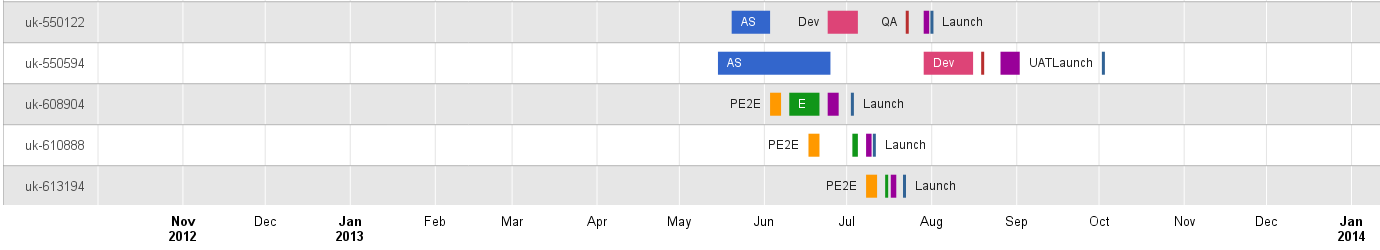
\includegraphics[width=1\textwidth]{./resources/report_timelines_new.png}
   	\caption{Timelines report}
   	\label{f_report_timelines_new}
\end{figure}

\subsection{The Output}
Once we put all reports together in a single page we obtain the following
result:

\begin{figure}[ht!]
	\centering
   	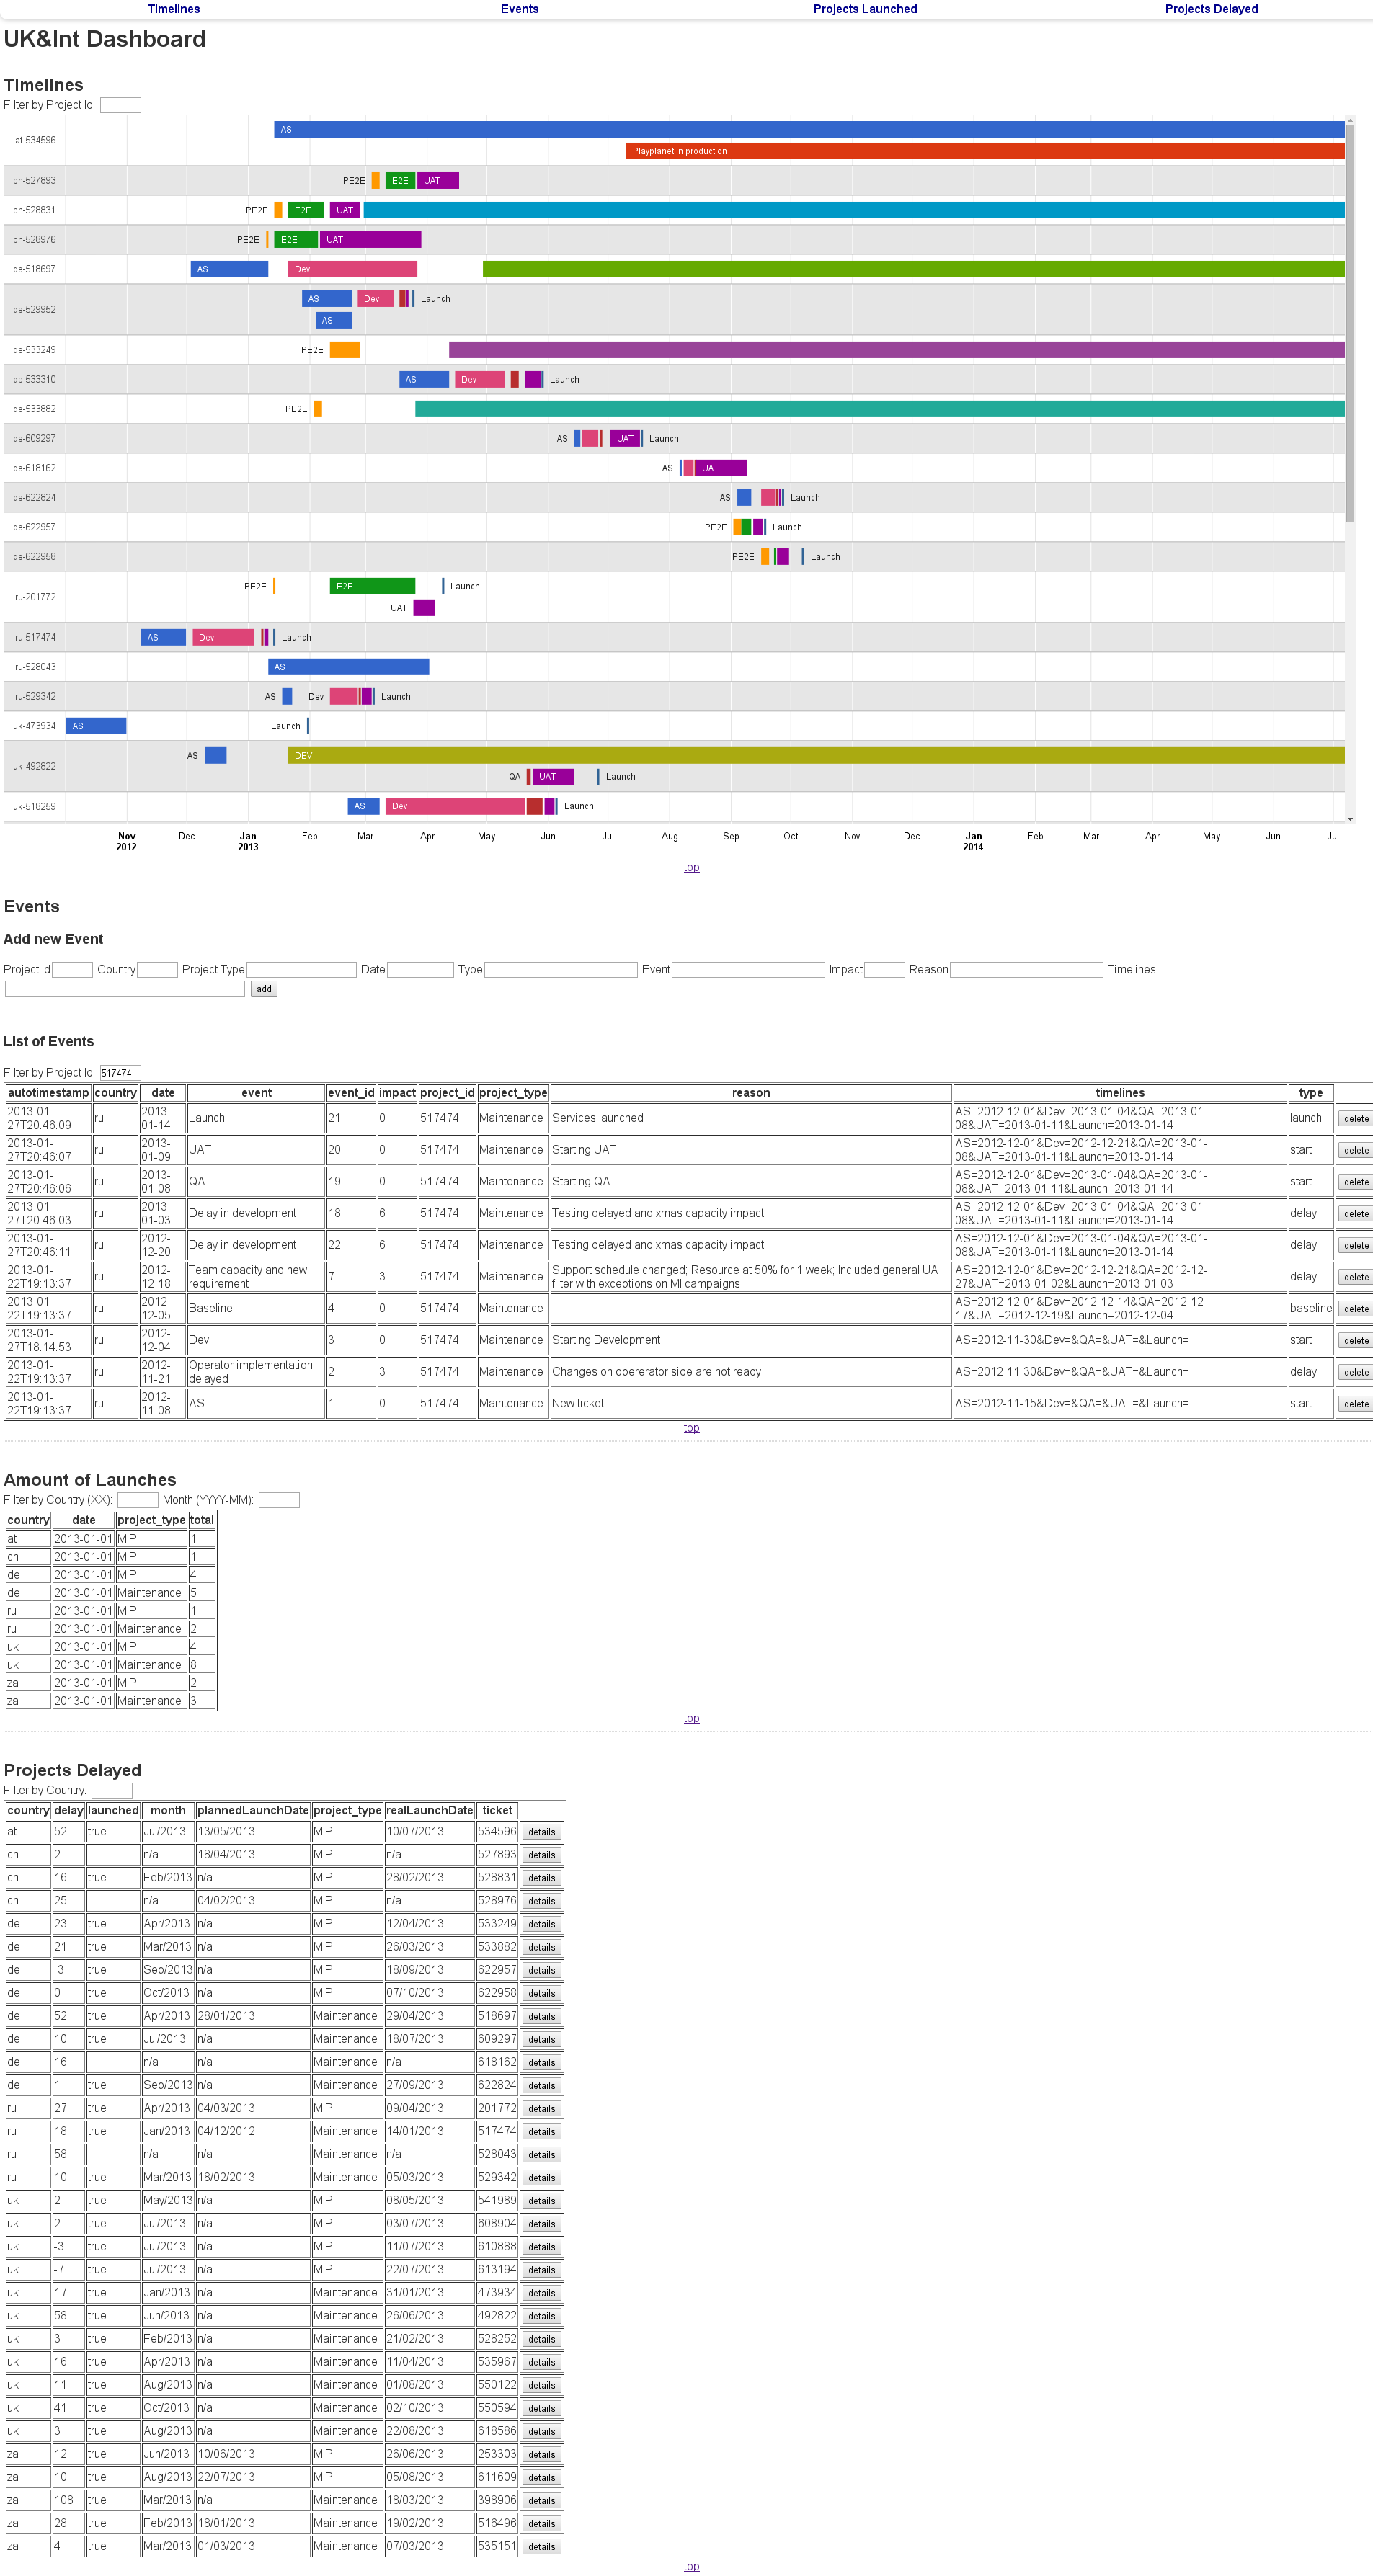
\includegraphics[width=0.9\textwidth]{./resources/dashboard.png}
   	\caption{http://dasboard.buongiorno.com}
   	\label{f_dashboard}
\end{figure}

%\begin{appendices}
%\chapter{Table views reports}
%\lstinputlisting[language=SQL,breaklines=true]{resources/reports_views.sql}
%\end{appendices}
